\documentclass[12pt,letterpaper,boxed]{hmcpset}
\usepackage{float}
\restylefloat{figure}
\usepackage{graphicx}
\usepackage{amsmath}


\name{Lujia Zhang}
\class{CSSE 477}
\mailbox{CM 1405}
\assignment{Assignment 10}

\begin{document}

\section*{Questions}
\begin{itemize}
  \item What is Semantic interoperability?
  \item How to implement and use Semantic interoperability?
  \item Why to use Semantic interoperability? What are the advantages?
\end{itemize}
\section*{Answers}
\begin{itemize}
  \item Semantic interoperability is the ability of software to share data between different system, clients and servers.
  \item In this lab, I used Google RPC to set up one Python server to response to both Python clients and Node Js client. Both clients can get the current time information from the server even though the programming languages can be different than the server language.
  \item Semantic interoperability is awesome to implement since the server and client can share information/data even with different programming language. The availability can be extended widely. And it's easy to add more clients.
  
\end{itemize}
\section*{Screen Shot}
I added extra PrintCurrentTimePython function in both python/node JS client side and server side so by calling the function, it will return the current time.

\begin{figure}[H]
  \centering
  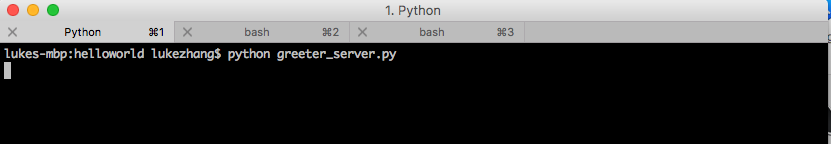
\includegraphics[width = 1.0\textwidth]{1.png}
  \caption{Python Server}
\end{figure}
\begin{figure}[H]
  \centering
  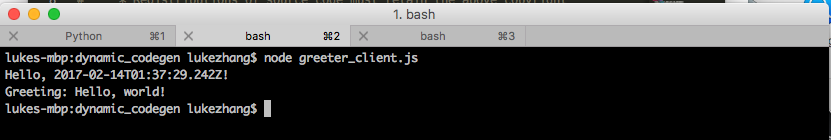
\includegraphics[width = 1.0\textwidth]{2.png}
  \caption{Node JS Client}
\end{figure}
\begin{figure}[H]
  \centering
  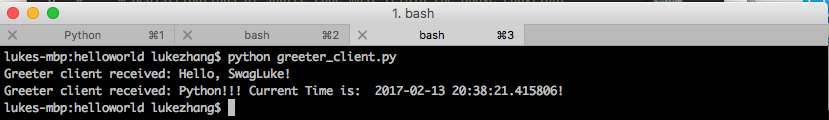
\includegraphics[width = 1.0\textwidth]{3.png}
  \caption{Python Client}
\end{figure}
\end{document}